% !TeX spellcheck = russian-aot
%\documentclass[12pt,a4paper,draft]{article}
%\usepackage{cmap}
%\usepackage[utf8]{inputenc}
%\usepackage[T2A]{fontenc}
%\usepackage[english,german,russian]{babel}
%\usepackage{amsmath}
%\usepackage{amsfonts}
%\usepackage{amssymb}
%\usepackage[final]{graphicx}
%\DeclareGraphicsExtensions{.jpg,.png}
%\graphicspath{{pictures/}} % путь к графическим файлам. Пусть они помещаются в подкаталог pictures текущего каталога
%\usepackage[figurename=Рисунок,labelsep=period]{caption}
%\usepackage{float}
%\usepackage{indentfirst}
%\usepackage[pdftex,left=2.5cm,right=2.5cm,top=3cm,bottom=3cm]{geometry}
%\usepackage[obeyDraft]{todonotes}
%\usepackage[hidelinks,draft=false]{hyperref}
%\frenchspacing
%\pdfcompresslevel=9

\documentclass[a4paper,12pt]{article}
\usepackage[utf8]{inputenc}
\usepackage[T2A]{fontenc}
\usepackage[english,russian]{babel}
\usepackage{natbib}
\usepackage[final]{graphicx}
\DeclareGraphicsExtensions{.jpg,.png}
\graphicspath{{pictures/}}
\usepackage{float}
\usepackage{amsmath}
\usepackage{pgfplots}
\usepackage{color} %% это для отображения цвета в коде
%\usepackage{listings} %% собственно, это и есть пакет listings




%\setmonofont{Consolas} %to be used with XeLaTeX or LuaLaTeX
\definecolor{bluekeywords}{rgb}{0,0,1}
\definecolor{greencomments}{rgb}{0,0.5,0}
\definecolor{redstrings}{rgb}{0.64,0.08,0.08}
\definecolor{xmlcomments}{rgb}{0.5,0.5,0.5}
\definecolor{types}{rgb}{0.17,0.57,0.68}

\usepackage{listings}
\lstset{
language=[Sharp]C,
captionpos=t,
%numbers=left, %Nummerierung
%numberstyle=\tiny, % kleine Zeilennummern
frame=lines, % Oberhalb und unterhalb des Listings ist eine Linie
showspaces=false,
showtabs=false,
breaklines=true,
showstringspaces=false,
breakatwhitespace=true,
escapeinside={(*@}{@*)},
commentstyle=\color{greencomments},
morekeywords={partial, var, value, get, set},
keywordstyle=\color{bluekeywords}\bf,
stringstyle=\color{redstrings},
basicstyle=\ttfamily\small,
extendedchars=\true
}

\usepackage{caption}
\DeclareCaptionFont{white}{\color{white}} %% это сделает текст заголовка белым
%% код ниже нарисует серую рамочку вокруг заголовка кода.
\DeclareCaptionFormat{listing}{\colorbox{gray}{\parbox{\textwidth}{#1#2#3}}}
\captionsetup[lstlisting]{format=listing,labelfont=white,textfont=white}


\usepackage{ctable}%для таблиц
\captionsetup[table]{justification=raggedleft,singlelinecheck=off}




%%%%%%%%%%%%%%%%%%%%%%%%%%%%%%%%%%%%%%%%%%%%%%%%%%%%%%%%%%%%%%%%%%%%%%%%%%%%%%%%%%%%%%%%%%%%%%%

\begin{document}
\begin{titlepage}
	\centering
    \begin{figure}[H]
    	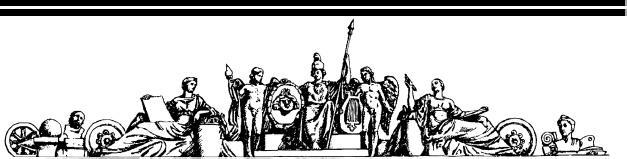
\includegraphics[scale=1.2]{photo}
   	\end{figure}
	{\scshape Министерство образования Российской Федерации
Московский Государственный Технический Университет им. Н.Э. Баумана \par}
	\vspace{4cm}
	{\scshape\Large Отчёт по лабораторной работе № 1\par}
    {\scshape\Large По курсу: "Анализ алгоритмов"\par}
	{\scshape\Large\bf Тема:"Муравьиный алгоритм."\par}
    \vspace{2cm}
    {\flushright Студент: Орехова Е.О. ИУ7-51\par
    \flushright Преподаватель: Волкова Л.Л.\par}
    \vspace{2cm}
% Bottom of the page
	{\large \today\par}
\end{titlepage}

\def\contentaname{Содержание}
\tableofcontents %Вывод содержания
\clearpage

\section{Постановка задачи}
    Реализовать муравьиный алгоритм на языке программирования. Сравнить работу алгоритма при разных значениях параметров задающих веса
    феромона и времени жизни колонии

\section{Идея}
    Муравьиный алгоритм - один из эффективных полиномиальных алгоритмов для
    нахождения приближённых решений задачи коммивояжёра, а также решения
    аналогичных задач поиска маршрутов на графах. Суть подхода заключается в анализе и
    использовании модели поведения муравьёв, ищущих пути от колонии к источнику питания
    и представляет собой метаэвристическую оптимизацию.
    С полным разбором алгоритма можно ознакомиться в книге М.В.Ульянова «Ресурсно-
    эффективные компьютерные алгоритмы. Разработка и анализ»
    
    Локальные правила поведения муравьев при выборе пути:
    \begin{itemize}
    	\item муравьи имеют собственную «память». Поскольку каждый город может
    	быть посещен только один раз, у каждого муравья сеть список уже посещенных городов — список запретов. Обозначим через $J_{i,k}$
    	список городов, которые необходимо посетить муравью k , находящемуся в городе i;
    	\item муравьи обладают «зрением» — видимость есть эвристическое желание
    	посетить город j , если муравей находится в городе i . Будем считать, что видимость обратно пропорциональна расстоянию между городами i и j - $D_{ij}$
    	\begin{equation}
    		\eta_{ij} = \frac{1}{D_{ij}};
    	\end{equation}
    	\item муравьи обладают «обонянием» — они могут улавливать след феромона,
    	подтверждающий желание посетить город j из города i, на основании опыта
    	других муравьев. Количество феромона на ребре (i,j) в момент времени t обозначим через $\tau_{ij}(t)$.
    \end{itemize}

	вероятность перехода k-ого муравья из города i в город j:
	\begin{equation}
	\begin{matrix}
	P_{ij,k}(t) & = 
	& \left\{
	\begin{matrix}
	\frac{[\tau_{ij}(t)]^\alpha * [\eta_{ij}]^\beta}{\sum\limits_{l = J_{i,k}} [\tau_{ij}(t)]^\alpha * [\eta_{ij}]^\beta }   & j \in J_{i,k} \\
	0 & j \notin J_{i,k} \\
	\end{matrix} \right. 
	\end{matrix}
	\end{equation}
	где $\alpha, \beta$ - коэффициенты, определяющие «стадность» алгоритма и «жадность» алгоритма).
	
	в конце каждого похода обновляется значение феромона на дорогах, используется следующая формула:
	\begin{equation}
	\tau_{ij}(t+1) = (1-p)*\tau_{ij}(t) + \Delta\tau_{ij}(t); \Delta\tau_{ij}(t) = \sum\limits_{k = 1}^{m} \Delta\tau_{ij,k}(t)
	\end{equation}
	
	где 
	\begin{equation}
	\begin{matrix}
	\Delta\tau_{ij,k}(t) & = \{
	\begin{matrix}
	\frac{Q}{L_k(t)}, & (i,j) \in T_k(t) \\
	0, & (i,j) \notin T_k(t) \\
	\end{matrix}
	\end{matrix}\}
	\end{equation}
	
	p - коэффициент испарения феромона; Q - параметр, имеющий значение порядка длины оптимального пути; $L_k$ - длина маршруту, пройденная муравьем k к моменту времени t; m - количество муравьев в колонии.
    
\section{Реализация}
\begin{lstlisting}[label=some-code,caption={Муравьиный алгоритм}]
static void gogo_ant(ref ant_t ant, matrix_t adj_mat, matrix_t weight, matrix_t d_pheromon, int q)
{
	int N = weight.n;
	int i = 1;
	int next = 0;
	array_t prob = create_array(N);
	while (i < N)
	{
		double sum_weight = 0;
		for (int j = 0; j < N; j++)
			sum_weight += weight.matr[ant.curr_city,j] * ant.Jk.arr[j];
		for (int j = 0; j < N; j++)
		{
			prob.arr[j] = weight.matr[ant.curr_city,j] / sum_weight * ant.Jk.arr[j];
		}
		next = choose_next(prob);
		ant.curr_city = next;
		ant.Jk.arr[next] = 0;
		ant.route.arr[i++] = next;
	}
	ant.Lk = (int)(length_of_route(adj_mat, ant.route));
	add_pheromon(d_pheromon, ant.route, ant.Lk, q);
}

static solution_t solve(matrix_t adj_mat, double a, double b, double p, int q, int t_max)
{
	int N = adj_mat.n;
	ant_t[] ants = create_ant_array(N); //array of ants, 1 per city;
	
	matrix_t pheromon = create_matrix(N, N);
	for (int i = 0; i < N; i++)
		for (int j = 0; j < N; j++)
			pheromon.matr[i,j] = 0.5;
	
	matrix_t visib = create_matrix(N, N);
	for (int i = 0; i < N; i++)
		for (int j = i; j < N; j++)
			if (i != j)
			{
				visib.matr[i,j] = 1 / adj_mat.matr[i,j];
				visib.matr[j,i] = visib.matr[i,j];
			}
			else
				visib.matr[i,j] = 1000;
	
	matrix_t weight = create_matrix(N, N);
	recalc_weight(ref weight, pheromon, visib, a, b);
	
	matrix_t d_pheromon = create_matrix(N, N);
	for (int i = 0; i < N; i++)
	for (int j = 0; j < N; j++)
	d_pheromon.matr[i,j] = 0;
	
	int best_l = int.MaxValue;
	array_t route = create_array(N);
	
	for (int t = 0; t < t_max; t++)
	{
		for (int k = 0; k < N; k++)
		{
			init_ant(ref ants[k]);
			gogo_ant(ref ants[k], adj_mat, weight, pheromon, q);
		}
		int best = -1;
		for (int i = 0; i < N; i++)
			if (ants[i].Lk < best_l)
			{
				best = i;
				best_l = ants[i].Lk;
			}
		if (best != -1)
		copy_array(route, ants[best].route);
		
		recalc_pheromon(ref pheromon, ref d_pheromon, p);
		recalc_weight(ref weight, pheromon, visib, a, b);
	}
	
	solution_t solv = new solution_t();
	solv.l = best_l;
	solv.route = route;
	return solv;
}
\end{lstlisting}

\section{Эксперимент}

\begin{figure}[H]
	\noindent\centering{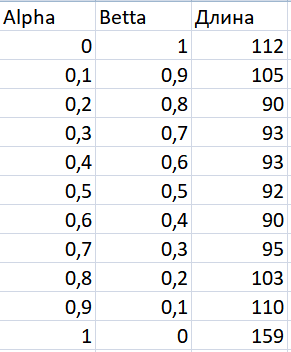
\includegraphics[scale = 1]{myr}}
	\caption{Поиск наименьшей длины в зависимости от $\alpha$ и $\beta$.}
	
	Наилучший результат алгоритм даёт при $\alpha = 0.6$ и $\beta = 0.4$.
	
	\noindent\centering{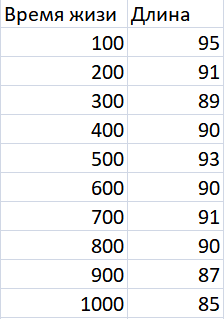
\includegraphics[scale = 1]{myr1}}
	\caption{Поиск наименьшей длины в зависимости от времени жизни колонии.}
	
	Увеличение времени жизни колонии приводит к лучшему результату.
	
\end{figure}

\section{Заключение}
	В ходе лабораторной работы был реализован муравьиный алгоритм,а также было
	проведено сравнение работы алгоритма при различных параметрах, задающих веса
	феромона и временя жизни колонии.
\end{document} 